% \section{Invalidity of Existing Methods for Weak-Instrument Robust Inference with Heterogeneous Treatment Effects}
\section{On the Validity of Existing Weak-instrument Robust Tests}
% Under Treatment Effect Heterogeneity

\label{sec:ar-clr}

In the following, we proceed to show that the \cite{andersonEstimationParametersSingle1949} AR test, the \cite{kleibergenGeneralizingWeakInstrument2007} LM test and the \cite{moreiraConditionalLikelihoodRatio2003} CLR test do not retain size under the combination of weak instruments and treatment effect heterogeneity, when \(d_Z>1\). We record the definitions of the statistics, in the notation \cite{finlayImplementingWeakInstrumentRobust2009}.
\begin{definitionp}{LEG}[Legacy Robust Test Statistics]
Let \(\hat\Omega(\beta_0) \equiv \hat\Sigma_{\hat\delta} - 2\beta_0\,\hat\Sigma_{\hat\delta,\hat\gamma} + \beta_0^2\,\hat\Sigma_{\hat\gamma}\) denote the variance of the restriction \(\hat \delta - \beta_0 \hat \gamma\), and let
\[\tilde\gamma(\beta_0) \equiv \hat\gamma - \hat\Omega(\beta_0) ^{-1}\bigl(\hat\Sigma_{\hat\delta,\hat\gamma} - \beta_0\,\hat\Sigma_{\hat\gamma}\bigr)\,(\hat\delta - \beta_0\hat\gamma)\] denote the first stage orthogonalized relative to \(\hat \delta - \beta_0 \hat \gamma\).
% normal projection of the restriction off the first stage. 
    \begin{enumerate}
        % \item[] 
        \item 
        The AR test statistic is defined as
        \begin{align}
        \mathrm{AR}(\beta_0) &\equiv \bigl\lVert (\hat\Omega(\beta_0)/n)^{-1/2}(\hat\delta - \beta_0\hat\gamma)\bigr\rVert^2
        \end{align}
        \item 
        The LM test statistic is defined as
        \begin{align}
        \mathrm{LM}(\beta_0) \;\equiv\; {\left[\tilde\gamma(\beta_0)'(\hat\Sigma(\beta_0)/n)^{-1}(\hat\delta - \beta_0\hat\gamma)\right]^2}\bigg/{\bigl\lVert(\hat\Sigma(\beta_0)/n)^{-1/2}\tilde\gamma(\beta_0)\bigr\rVert^2}.
        \end{align}
        \item 
        The CLR test statistic is defined as
        % \begin{align}
        % \end{align}
        \begin{align}
        \mathrm{CLR}(\beta_0) = \frac{1}{2}\left[AR(\beta_0) + \sqrt{(AR(\beta_0)-\hat r(\beta_0))^2 + 4 \cdot LM(\beta_0) \cdot \hat r(\beta_0)} \right] 
    \end{align}
    \end{enumerate}
    \noindent 
     where \(\hat r(\beta_0) \equiv \bigl\lVert(\hat\Sigma(\beta_0)/n)^{-1/2}\tilde\gamma(\beta_0)\bigr\rVert^2\). The Sargan-Hansen J-statistic is defined as \(\hat J(\beta_0)\equiv AR(\beta_0)- LM(\beta_0)\).
    % Ob Sargan-Hansen J test is defined as \(\hat J(\beta_0)\equiv \ldots\). Observe that \( = + J(\beta_0)\).
\end{definitionp}
% \begin{align*}
% ,
% \end{align*}
% and let $\hat P(\beta_0)$ denote the rank-1 orthogonal projector onto $\mathrm{span}\bigl((\hat\Omega(\beta_0)/n)^{-1/2}\tilde\gamma(\beta_0)\bigr)$, i.e.\
% \[
% \hat P(\beta_0) \;:=\; \frac{\hat w(\beta_0)\,\hat w(\beta_0)'}{\hat w(\beta_0)'\hat w(\beta_0)}, \qquad \hat w(\beta_0) := (\hat\Omega(\beta_0)/n)^{-1/2}\tilde\gamma(\beta_0).
% \]
% Then
% \begin{align*}
% ,\\
% \mathrm{LM}(\beta_0) &\equiv \bigl\lVert \hat P(\beta_0)\,(\hat\Omega(\beta_0)/n)^{-1/2}(\hat\delta - \beta_0\hat\gamma)\bigr\rVert^2,\\
% % \mathrm{J}(\beta_0) &\equiv \bigl\lVert \bigl(I_{d_Z} - \hat P(\beta_0)\bigr)\,(\hat\Omega(\beta_0)/n)^{-1/2}(\hat\delta - \beta_0\hat\gamma)\bigr\rVert^2.
% \end{align*}
% We can show that t
% The three tests are closely related. We see this by considering the following identities.
% \begin{lemmap}{LEG-ID}[Legacy Identities]
% \begin{enumerate}
%     \item[] 
%     \item 
%     The AR, LM and J tests are related as follows:
%     \begin{align}
%         AR(\beta_0) = LM(\beta_0) + J(\beta_0)
%     \end{align}
%     \item 
%     The CLR, LM and J tests are related as follows:
%     \begin{align}
%         CLR(\beta_0) = \frac{1}{2}\left[AR(\beta_0) + \sqrt{(AR(\beta_0)-\hat r)^2 + 4 \cdot LM(\beta_0) \cdot \hat r} \right] 
%     \end{align}
%     where \(\hat r\equiv \ldots\) is a feature of the sample.
% \end{enumerate}
% \end{lemmap}
% \begin{proof}
%     % See \cite{finlayImplementingWeakInstrumentRobust2009}.
%     See Appendix X.
% \end{proof}
% \noindent
\noindent
With constant effects, we have the following limiting distributions.
\begin{lemmap}{LEG-CTE}[Legacy tests, Constant Treatment Effects] Assume there exists a scalar \(\beta\) such that \(\delta_n=\beta \gamma_n\). We then have, uniformly, the following limits.
    \begin{enumerate}
        % \item[] 
        \item 
        \(\mathrm{AR}(\beta_0)\convd \mathfrak{C}^2_{d_Z}\)
        \item 
        \(\mathrm{LM}(\beta_0)\convd \mathfrak{C}^2_1\)
        \item 
        \(\mathrm{LR}(\beta_0)\convd \frac{1}{2}\left[\mathfrak{C}^2_{d_Z-1}+\mathfrak{C}^2_1 + \sqrt{(\mathfrak{C}^2_{d_Z}+\mathfrak{C}^2_1)^2 + 4 \cdot \mathfrak{C}^2_1 \cdot \hat r} \right]\) 
    \end{enumerate}
\end{lemmap}
\begin{proof}
    % See \cite{finlayImplementingWeakInstrumentRobust2009}.
    See Appendix X.
\end{proof}
\noindent
With treatment effect heterogeneity, this result no longer obtains.
\begin{lemmap}{LEG-HTE}[Legacy tests, Heterogeneous Treatment Effects] Assume there exists a scalar \(\beta\) such that \(\delta_n=\beta \gamma_n\). Then, we have:
    \begin{enumerate}
        % \item[] 
        \item 
        \(\mathrm{AR}(\beta_0)\convd \mathfrak{C}^2_{d_Z}(\lambda_{\mathrm{AR}})\)  where \(\lambda_{\mathrm{AR}} = \frac{\mu^2}{\mu^2+\eta^2} \cdot \nu^2\)
        \item 
        \(\mathrm{LM}(\beta_0)\convd \mathfrak{C}^2_1(\lambda_{\mathrm{LM}})\) where \(\lambda_{\mathrm{LM}} = \frac{\eta^2\,\mu^2\,\nu^2}{(\mu^2+\eta^2)[(\mu^2+\eta^2)^2 + \eta^2\,\nu^2]} \cdot \nu^2\)
        \item 
        \(\mathrm{J}(\beta_0)\convd \mathfrak{C}^2_{d_Z-1}(\lambda_{\mathrm{J}})\)  where \(\lambda_{\mathrm{J}} = \frac{\mu^2(\mu^2+\eta^2)}{(\mu^2+\eta^2)^2 + \eta^2\,\nu^2} \cdot \nu^2\)        
        \item 
        \(\mathrm{LR}(\beta_0)\convd \frac{1}{2}\left[\mathfrak{C}^2_{d_Z-1}(\lambda_{\mathrm{J}})+\mathfrak{C}^2_1(\lambda_{\mathrm{LM}}) + \sqrt{(\mathfrak{C}^2_{d_Z-1}(\lambda_{\mathrm{J}})+\mathfrak{C}^2_1(\lambda_{\mathrm{LM}}))^2 + 4 \cdot \mathfrak{C}^2_1(\lambda_{\mathrm{LM}}) \cdot \hat r} \right]\) 
    \end{enumerate}
    % It follows that tests based on these statistics will be centered away from zero, and hence not be uniformly valid when X, Y and Z.
    \noindent
where \(\mu^2,\nu^2\) and \(\eta^2\) are as defined in the previous section.
\end{lemmap}
\begin{proof}
    See Appendix X.
\end{proof}
\begin{remark} 
We make two observations.
\begin{enumerate}
    \item 
    AR and CLR are centered away from zero whenever \(\nu^2>0\), i.e. in the presence of heterogeneous treatment effects. The result holds in the limit as \(\mu^2\to\infty\). 
    \item 
    LM  is centered away from zero whenever \(\nu^2>0\) and \(\mu^2<\infty\). The test is centered at zero in the limit as \(\nu^2>0\) if \(\mu^2\to\infty\).    
\end{enumerate}
As a consequence, neither AR, CLR or LM are valid tests under the combination of weak instruments and treatment effect heterogeneity.
\end{remark}
\noindent 
% \noindent
In \Cref{fig:other-tests}, we plot the size of the AR, LM and CLR tests, used as as (quasi-)tests for the TSLS hypothesis  \(\beta=\beta_0\), under the assumption of constant effects, and with treatment effect heterogeneity.
% different tests for \(\beta=\beta_0\), where \(\beta\) denotes the TSLS estimand, under constant effects and under heterogeneous treatment effects. 
In panel (a), we see that the AR, LM and CLR tests are valid with constant treatment effects at every level of instrument strength. In panel (b), we see that with treatment effect heterogeneity,  all three tests overreject. We see that the degree of overrejection is increasing in instrument strength for AR and CLR and decreasing for LM. 
% Formally, this is because the distributions of the test statistics are now centered away from zero. Intuitively, it is because the heterogeneous effects are more strongly identified from the sample as the strength of the instrument grows.
% The figure also illustrates that the Wald tests derived from the TSLS and Jackknife IV estimators are both invalid with constant and heterogeneous treatment effects when the instrument set is weak.
\begin{figure}[!htb]
    \centering
    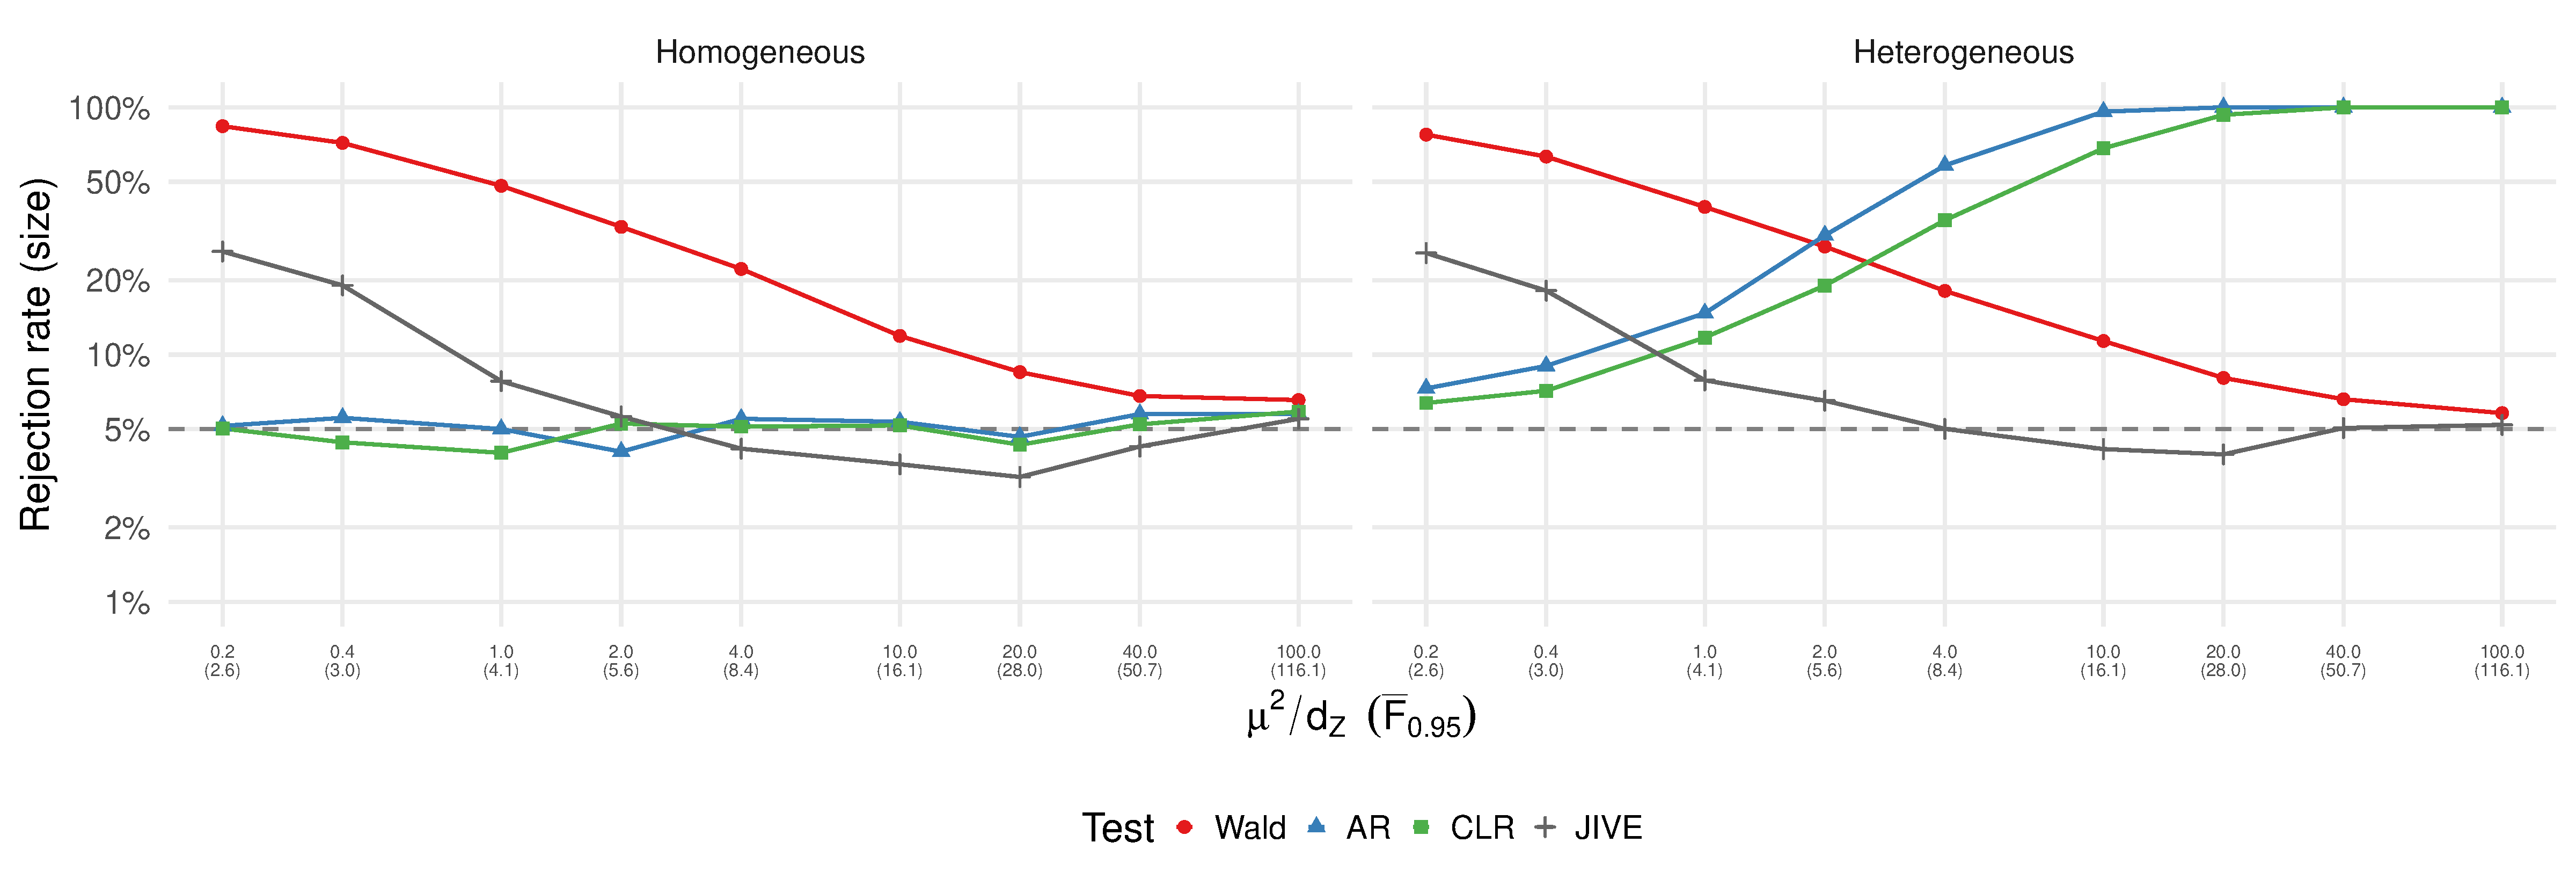
\includegraphics[width=\textwidth]{figs/inference_size_dz5_rho0.999.pdf}
    \caption{\textbf{Overrejection of the Wald, AR and CLR Tests Under Heterogeneous Treatment Effects} This figure plots the rate of over-rejection of the hypothesis \(\beta=\beta_0\) when \(\beta\) is homogeneous, and when it is the TSLS/JIVE estimand (heterogeneous treatment effects), with weak instruments. The red line shows the Wald test, the blue line the \cite{andersonEstimationParametersSingle1949} AR test and the green line the \cite{moreiraConditionalLikelihoodRatio2003} CLR test. The y axis shows the rejection rate (size), and the x axis enumerates instrument strength.}
    \label{fig:other-tests}
\end{figure}

% \noindent
% With respect to tests that are valid with many, potentially weak, instruments, we refer to \cite{yapInferenceManyWeak2025}, which to the author's knowledge derive the first such test that is valid under heterogeneous treatment effects.

% is the Wald test, which is valid with strong instruments, but as is shown by \cite{staigerInstrumentalVariablesRegression1997} does not retain size when instruments are weak. The second is the \cite{ander}

% \begin{enumerate}
%     \item 
%     Review argument against AR and CLR
% \end{enumerate}

% \clearpage 


% Thus far, we have considered estimators of some weighted average of local average treatement effects. However, existing approaches to inference also are lacking in the face of heterogeneous effects and weak instruments. In the following, we derive a test that is uniformly valid under heterogeneous treatment effects and weak instruments. \cite{yapInferenceManyWeak2025} has derived a test which is valid with many weak instruments and heterogeneous effects, but this relies on many-instrument asymptotics. We focus on the setting with a fixed number of instruments. We start by considering why the AR and CLR tests are invalid under heterogeneous effects. We then consider when we can reasonably assume to have ``many'' instruments. We lastly turn to deriving our preferred test.

% \subsection{Why AR and CLR do not work}

% % Let \((\hat \delta,\hat \gamma)\) be the OLS estimators of \((\delta_n,\gamma_n)\). Note that these are defined irrespective of whether their probability limits vary with the data generating process or not. Let \(\Sigma\) denote their joint variance covariance matrix, such that
% % \begin{align*}
% %     \begin{bmatrix}
% %         \sqrt{n}\,(\hat \delta - \delta_n) \\
% %         \sqrt{n}\,(\hat \gamma - \gamma_n) \\
% %     \end{bmatrix}
% %     \convd 
% %     \mathfrak{N}\left(\mathbf{0}_{2d_Z},\Sigma\right) 
% %     \qquad 
% %     \Sigma   \equiv 
% %    \begin{bmatrix}
% %        \Sigma_{\hat \delta} & \Sigma_{\hat \delta,\hat \gamma} \\ 
% %        \Sigma_{\hat \delta,\hat \gamma}' & \Sigma_{\hat \gamma}
% %    \end{bmatrix}
% % \end{align*}
% % where  the \(d_Z \times d_Z\) dimensional asymptotic variance- and covariance matrices of \((\hat \delta,\hat\gamma)\).\footnote{
% % I.e.,

% % \(\Sigma_{\hat\delta} \equiv \Sigma_{ZZ}^{-1}\, \E[\tilde Z_i\tilde Z_i' W_i^2]\, \Sigma_{ZZ}^{-1}\), 
% % \(\Sigma_{\hat\gamma} \equiv \Sigma_{ZZ}^{-1}\, \E[\tilde Z_i\tilde Z_i' V_i^2]\, \Sigma_{ZZ}^{-1}\) and
% % \(\Sigma_{\hat\delta,\hat\gamma} \equiv \Sigma_{ZZ}^{-1}\, \E[\tilde Z_i\tilde Z_i' W_i V_i]\, \Sigma_{ZZ}^{-1}\).
% % }
% % Let \(\Sigma_{ZZ} \equiv \E[\tilde Z_i\tilde Z_i']\), and let \(\hat \Sigma_j\) denote a sample analog estimator of \(\Sigma_j\). 

% The \cite{andersonEstimationParametersSingle1949} AR test is a test of the restriction
% \begin{align}
%     \mathcal{H}_0: \delta_n - \beta_0 \gamma_n = 0
% \end{align}
% For \(d_Z=1\), this is a scalar restriction, in a linear model equivalent to \(\beta=\beta_0\). for \(d_Z\geq 2\), it is equivalent to the joint restriction
% \begin{align}
%     \mathcal{H}_0: \beta = \beta_0 \qquad \land  \qquad \delta_n = \beta \gamma_n 
% \end{align}
% which amounts to \(d_Z\) different restrictions. Let \(\delta_j\) and \(\gamma_j\) denote the elements of \(\delta_n\) and \(\gamma_n\).
% There are \(d_Z\) restrictions that \(\delta_j = \beta \gamma_j\) for some \(\beta\), and one restriction that this beta is \(\beta=\beta_0\). The latter restriction can be subsumed into the former, and so in total it is a restriction of \(d_Z\) degrees of freedom. As a consequence, the AR test can reject either because \(\beta\neq \beta_0\), or because \(\delta_j \neq \beta \gamma_j\) for all \(j=1,\ldots,d_Z\), for the same scalar \(\beta\). The interpretation of the latter can be one of two: If the researcher maintains a constant-effects assumption, it implies a violation of instrument exogeneity. This is known as an ``overidentification test''~\citep{sarganEstimationEconomicRelationships1958,hansenLargeSampleProperties1982}. Otherwise, it can be considered a rejection of constant effects.

% One way to see that the AR test works this way is the observation by \cite{moreiraConditionalLikelihoodRatio2003}, as summarized in \cite{finlayImplementingWeakInstrumentRobust2009}, that the AR test statistic can be broken up into two parts. In particular:
% \begin{align}
%     AR(\beta_0) = LM(\beta_0) + J(\beta_0)
% \end{align}
% where \(LM(\beta_0)\) is the \cite{kleibergenGeneralizingWeakInstrument2007} LM score test and \(J(\beta_0)\) is the Sargan-Hansen J-statistic for overidentification. \cite{moreiraConditionalLikelihoodRatio2003} derived a more powerful test which overcome the challenges to power induced by the two joint hypotheses. The interpretation of his CLR test is that it tests \(\beta=\beta_0\)  against \(\beta\neq \beta_0\) while maintaining the assumption that there exists some scalar \(\beta\) such that \(\delta_n = \beta \gamma_n\) both under the null and the alternative. 

% In \Cref{fig:other-tests}, we plot the rejection rate for \(\beta=\beta_0\) at the true \(\beta\) 
% \begin{figure}[!b]
%     \centering
%     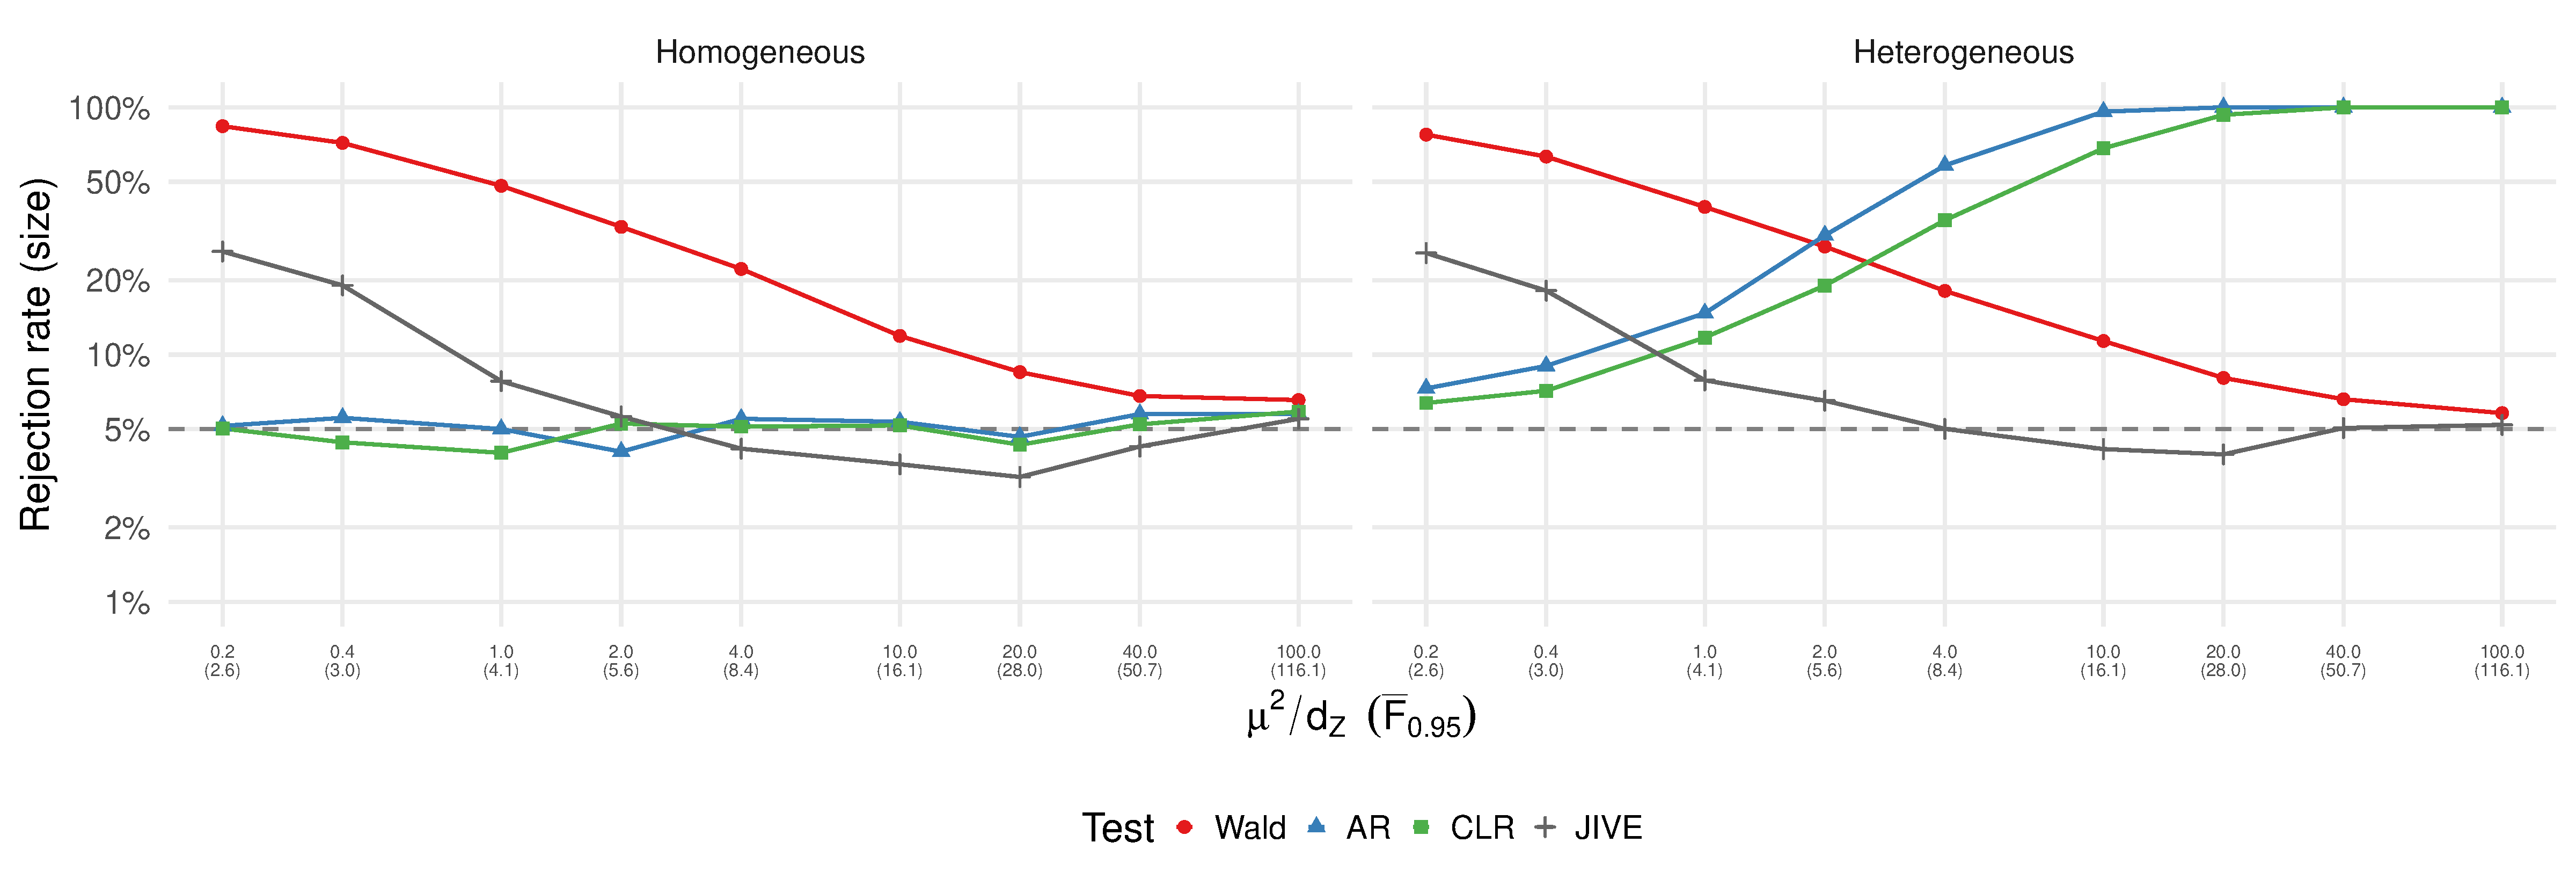
\includegraphics[width=\textwidth]{figs/inference_size_dz5_rho0.999.pdf}
%     \caption{\textbf{Overrejection of the Wald, AR and CLR Tests Under Heterogeneous Treatment Effects} This figure plots the rate of over-rejection of the hypothesis \(\beta=\beta_0\) when \(\beta\) is homogeneous, and when it is the TSLS/JIVE estimand (heterogeneous treatment effects), with weak instruments. The red line shows the Wald test, the blue line the \cite{andersonEstimationParametersSingle1949} AR test and the green line the \cite{moreiraConditionalLikelihoodRatio2003} CLR test. The y axis shows the rejection rate (size), and the x axis enumerates instrument strength.}
%     \label{fig:other-tests}
% \end{figure}
% for the TSLS and JIVE Wald tests, the AR test and the CLR test in the case of \(d_Z=10\) instruments, for different instrument strengths, \(\mu^2/d_Z\). We see that the TSLS and JIVE Wald tests over-rejects for weak instruments, but is consistent in level as instrument strength increases, both under constant and heterogeneous treatment effects. On the other hand, AR and CLR are consistent in level under constant effects, but not under heterogeneous treatment effects.

% Note that the JIVE Wald test is valid for moderate instrument strengths, but not uniformly. Further, it is conservative for intermediate values of the concentration parameter. This justifies looking for a better test statistic.

% \subsection{When are instruments ``many''?}

% Another strand of the literature has focused on deriving tests that are valid under many instruments or many weak instruments. \cite{evdokimovInferenceInstrumentalVariables2018} derive test statistics based on the TSLS and Jackknife IV estimator that are consistent in level when there are potentially many instruments and heterogeneous treatment effects. 
% \cite{mikushevaInferenceManyWeak2022} to derive a ``Jackknife AR'' test statistic that is consistent under many weak instruments, but which is not valid under heterogeneous treatment effects. 
% \cite{yapInferenceManyWeak2025} build on both papers to derive an LM-Score statistic that is consistent in level with many weak instruments and heterogeneous treatment effects.


% A relevant question when considering these tests is when we believe that we have ``many'' instruments. Formally, the papers in this literature consider sequences of data-generating processes where the number of instruments go to infinity, \(d_Z\to\infty\) as \(n\to\infty\), either in such a way that \(d_Z/n\to c<\infty\) or \(\mu^2/d^{k}_Z \to c<\infty\) for some \(k\in\{1/2,1\}\). One of the approximations used in this literature, e.g. by \cite{mikushevaInferenceManyWeak2022}, is the limiting result that as \(d_Z\to\infty\), we have
% \begin{align}
%     (\mathfrak{C}^2_{d_Z}-d_Z)/\sqrt{2d_Z} \convd \mathfrak{N}(0,1) 
% \end{align}
% i.e. that the demeaned and scaled chi-squared distribution converges to a standard normal. In order to evaluate this approximation, in \Cref{fig:chi2-convergence}, we plot the degree of over-rejection of the test statistic  \((d_Z\hat F - d_Z)/\sqrt{2d_Z}\) when asymptotically compared to its normal approximation, relative to when it is compared to its true, fixed-\(d_Z\) limiting distribution. We see that even at \(d_Z=100\) we still have 14\% over-rejection at level \(\alpha=0.05\). As such, we conclude that methods derived in the ``many weak instruments'' regime need not necessarily extend to the fixed-\(d_Z\) weak instruments regime.


% \begin{figure}[!htb]
%     \centering
%     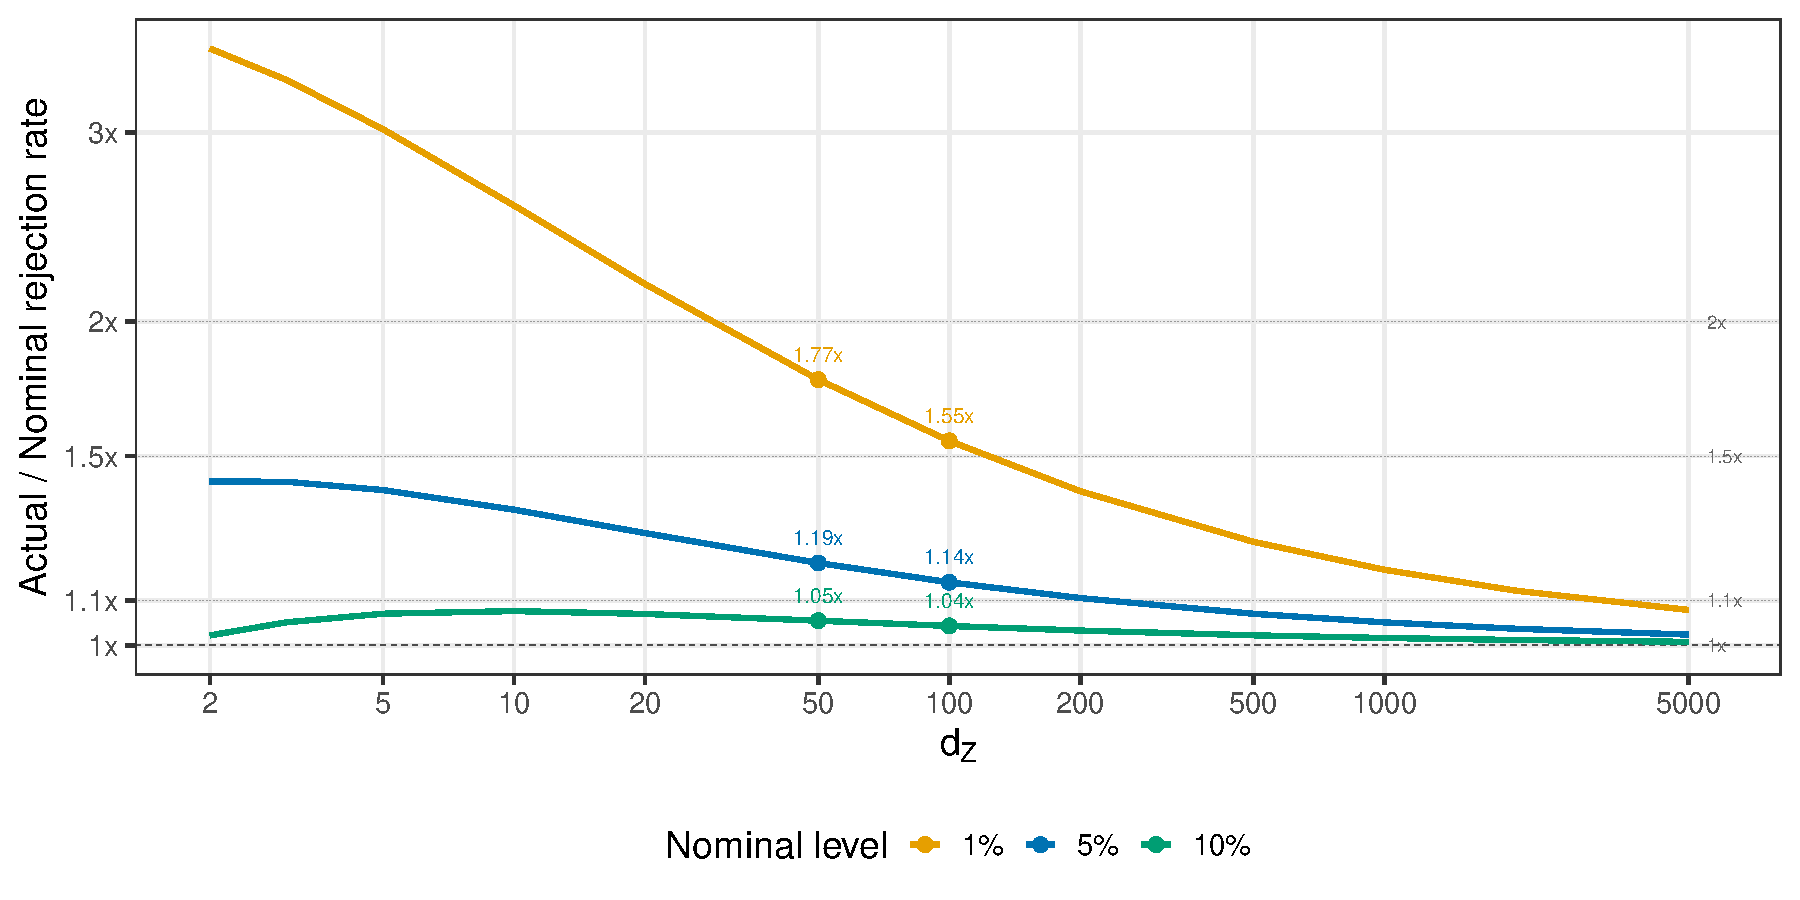
\includegraphics[width=0.9\linewidth]{figs/chi2_normal_overrejection_ratio.pdf}
%     \caption{\textbf{Overrejection of the Normal-approximated adjusted First-stage F-statistic} This figure plots the rate of over-rejection of the hypothesis \(\gamma_n=0\) using the test statistic \(\hat F-1\) and using the standard normal distribution as limiting distribution in place of its true distribution, \((\mathfrak{C}^2_{d_Z}-d_Z)/d_Z\). It is informative of how fast ``many instruments'' asymptotics kick in.}
%     \label{fig:chi2-convergence}
% \end{figure}


% \begin{align}
%     \Gamma(\beta_0) = \begin{pmatrix} 0 & \Sigma_{ZZ} \\ \Sigma_{ZZ} & -2\beta_0\Sigma_{ZZ}\end{pmatrix}
% \end{align}
% \begin{align}
%     \Sigma 
% \end{align}